\documentclass[12pt]{article}

\usepackage{amssymb,amsmath,amsthm}
\usepackage{graphicx} % Package for including figures
%\usepackage{psfrag,color}

\theoremstyle{definition}
\newtheorem{thm}{Theorem}[section]
\newtheorem{lem}[thm]{Lema}
\newtheorem{prop}[thm]{Proposition}
\newtheorem*{cor}{Corrolary}

\theoremstyle{definition}
\newtheorem{defn}{Definition}[section]
\newtheorem{conj}{Conjecture}[section]
\newtheorem{exmp}{Example}[section]


\title{Report: Homework 4 Math/CS 471}
\author{Teo Brandt and Brennan Collins}
\date{\today}   % Activate to display a given date or no date


\begin{document}
\maketitle

\begin{abstract}
This report will demonstrate the methods used to approximate derivatives and integrals on a closed domain \OMEGA with respect to some reference domain \(\OMEGA_{R}\). In general, the places (domains) we wish to solve are not described by explicit formulas of the geometry, so these methods are useful in dealing with multidimensional problems that are observed in reality.
\end{abstract}

\section{Approximating Derivatives}
One obvious choice is to compute the spatial derivatives using finite differences \(\frac{\delta u}{\delta x} (x) \approx \frac{u(x+h)-u(x)}{h}\). However, if the domain does not really correspond to the x and y axis exactly it is useful to apply the chain rule. Some examples of simple domains are displayed in the figures below.
\begin{figure}[htp]

\centering
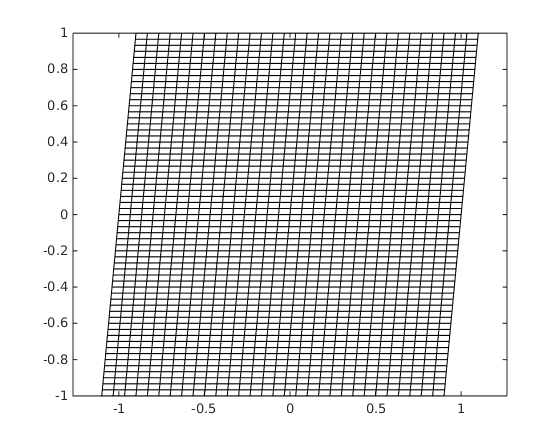
\includegraphics[width=.3\textwidth]{result1}\hfill
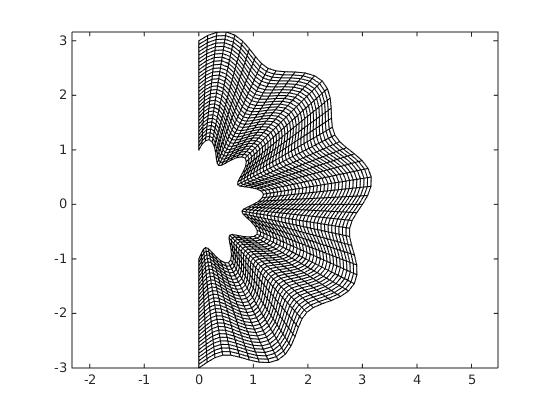
\includegraphics[width=.3\textwidth]{result2}\hfill
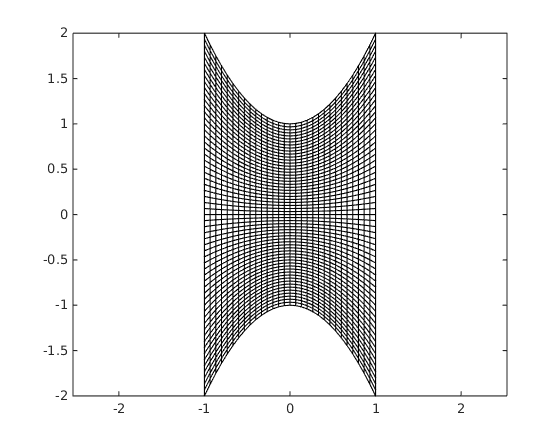
\includegraphics[width=.3\textwidth]{result3}

\caption{Combinations 1-3}
\label{fig:figure3}

\end{figure}
%\begin{figure}[h]
%\caption{Combination 1}
%\centering
%\includegraphics[scale = 0.5]
%{result1}
%\end{figure}
%\\
%\begin{figure}[h]
%\caption{Combination 2}
%\centering
%\includegraphics[scale = 0.5]
%{result2}
%\end{figure}
%\\
%\begin{figure}[h]
%\caption{Combination 3}
%\centering
%\includegraphics[scale = 0.5]
%{result3}
%\end{figure}
\\
For example if we would like to approximate \(\frac{\delta g(x,y)}{\delta x}\) we use the chain rule to find
\[
\frac{\delta u}{\delta x} = \frac{\delta r}{\delta x} *\frac{\delta u}{\delta r} +\frac{\delta s}{\delta x} *\frac{\delta u}{\delta s} 
\]
and similarly for
\[
\frac{\delta u}{\delta y} = \frac{\delta r}{\delta y} \frac{\delta u}{\delta r} +\frac{\delta s}{\delta y} \frac{\delta u}{\delta s} 
\]
where \(\frac{\delta u}{\delta r}\) and \(\frac{\delta u}{\delta s}\) are found using standard finite difference formulas.To find the metric \(r_{x}\), \(r_{y}\), \(s_{x}\), \(s_{y}\) we can first compute \(x_{r}\), \(x_{s}\), \(y_{r}\), \(y_{s}\) and then use the above formulas with \(u=x\) and \(u=y\). This yields
\[
\begin{bmatrix}
    r_{x}       & s_{x} \\
    r_{y}       & s_{y}
\end{bmatrix}
\begin{bmatrix}
    x_{r}       & y_{r} \\
    x_{s}       & y_{s}
\end{bmatrix}
=
\begin{bmatrix}
    1       & 0 \\
    0       & 1
\end{bmatrix}
\]
By solving the above relation analytically the following expressions were derived
\[
s_{x}=\frac{-y_{r}}{x_{r}y_{s}-x_{s}y_{r}}; s_{y}=\frac{x_{r}}{x_{r}y_{s}-x_{s}y_{r}}; r_{x}=\frac{y_{s}}{x_{r}y_{s}-x_{s}y_{r}}; r_{y}=\frac{-x_{s}}{x_{r}y_{s}-x_{s}y_{r}}
\]

\section{Compute Integrals}
To compute integrals on the reference element we break the domain integral down as shown
\[
\int_{\OMEGA}f(x,y)dxdy=\int\int f(x(r,s),y(r,s))J(r,s)drds,
\]
Where \(J(r,s)=x_{r}y_{s}-x_{s}y_{r}\) is the surface element \cite{HW}. One method that was used in the previous report, and can be used here is the trapezoidal rule, shown below
\[
\int_{X_{L}}^{X_R}f(x)dx\approx h\bigg(\frac{f(x_{0})+f(x_{n})}{2}+\sum_{i=1}^{n-1}f(x_{i})\bigg)
\]
where the grid is given by \(x_{i}=X_{L}+ih\text{, }i=0,...,n\text{, }h=\frac{X_{R}-X_{L}}{n}\).

\section{Results and Findings}
Using the first combination with \(x_{coord} = r+0.1d0*s, y_{coord} = s,\text{ and} u = sin(xc)*cos(yc)\), we know that the area should be \((r_{n}-r_{0})*(s_{n}-s_{0}) = (1-(-1)) * (1-(-1)) = 2*2 = 4\). Using trapezoidal approximation, we found that the area was 3.9999999999999996, which is just about equal to 4.
%\section{Results}
%\begin{figure}[h]
%\caption{Plot of error against \textbf{n}}
%\centering
%\includegraphics
%{error_plot}
%\end{figure}
%\\
%In the figure shown above, different rates of convergence are observed for each of the methods and for each of the values of \(k\). The trapezoidal method where \(k=\pi^{2}\) is the only case in which the order of the method may be read from the slope of its plot. This slope is \(\approx -3\) which is consistent with the theory as shown for
\newpage
\section{Appendix}
\indent In order to compile and execute the code for this assignment a make file is used:
\\
\begin{center}
\textit{~/Homework/Homework4/Code/}
\end{center}
\\
Once in this directory the following command will compile and execute the code:
\\
\begin{center}
\textit{\$ make \&\& ./homework4.x}
\end{center}
\\

\newpage
\begin{thebibliography}{9}
\bibitem{HW} 
Daniel Appelo
\textit{Homework 3}. 
referenced Sep. 26, 2015

\end{thebibliography}

\end{document} 